\documentclass[journal]{IEEEtran}

\usepackage[T1]{fontenc}
\usepackage[utf8]{inputenc}
\usepackage{cite}
\usepackage{amsmath,amssymb}
\usepackage{graphicx}
\usepackage{booktabs}
\usepackage{tabularx}
\usepackage{array}
\usepackage{url}
\usepackage[hidelinks]{hyperref}
\usepackage{fontawesome5}
\usepackage{tikz}
\usetikzlibrary{arrows.meta,positioning,fit}

\newcommand{\WER}{\mathrm{WER}}
\newcolumntype{Y}{>{\raggedright\arraybackslash}X}

\title{Domain Adaptation and Conservative Hypothesis Consensus for Code-Switched Indonesian--Javanese Speech Recognition: A Competition Case Study}

\author{Aakash Balasubramanian and Aniruth Devaraj\quad\href{https://github.com/06-aakash-06/lost-in-transcription}{\faGithub}%
\thanks{The authors are with the Department of Computer Science and Engineering, Sri Sivasubramaniya Nadar College of Engineering, Kalavakkam, Chennai, Tamil Nadu, India.}%
}

\begin{document}
\maketitle

\begin{abstract}
Spontaneous Indonesian--Javanese speech brings together within-utterance language switching, colloquial forms, disfluencies, long clips, and variable spelling. This paper documents our end-to-end response to the Indonesian--Javanese Lost in Transcription task: audit and prepare the supplementary Jember corpus, adapt Whisper large-v3-turbo and MERaLiON with low-rank updates, compare their outputs on conversation-disjoint development folds, and restrict fusion edits to cases supported by two model outputs. The labelled development set contains 372 clips from two conversations and four speakers; the audited Jember set contributes 1,309 training chunks and 162 session-held-out chunks. The selected conservative Turbo submission reached final displayed leaderboard values of 0.2712 and 0.2743 and a team-reported rank of 34th among 500 entries. Those displayed values are kept separate from local word error rate (WER) because the archived screenshot did not preserve their column headings. In a later offline experiment, Whisper large-v3 reduced aggregate conversation-disjoint WER from 0.199943 alone to 0.193938 with deterministic, unambiguous word-level consensus. That later result was not submitted and has no measured leaderboard score. The findings favor a strong adapted anchor and bounded corrections, while the small number of development conversations limits claims of generalization.
\end{abstract}

\begin{IEEEkeywords}
automatic speech recognition, code-switching, Indonesian, Javanese, low-resource speech, parameter-efficient adaptation, hypothesis consensus
\end{IEEEkeywords}

\section{Introduction}
In a spontaneous bilingual conversation, a speaker can move between languages without pausing to announce the change. The recognizer must follow those changes while also handling informal pronunciation, fillers, repetitions, names, and spelling conventions. These conditions make exact-match evaluation difficult: a transcript can preserve a speaker's meaning and still incur word errors when it chooses a different lexical form.

This study follows our work on the Indonesian--Javanese track of the Lost in Transcription competition. We began with heterogeneous recognizers and voting, then shifted toward a domain-adapted Whisper anchor after local development results did not predict the first completed competition result. We adapted Whisper large-v3-turbo and MERaLiON, tested whether their hypotheses could help one another, and eventually allowed only short substitutions supported by both alternatives. A later Whisper large-v3 experiment is reported as offline research and is not credited with the competition result.

The paper makes three bounded contributions. First, it records the data audit and conversation-disjoint validation used to adapt models with a small supplementary corpus. Second, it compares model and fusion variants, including cases where fusion helped and harmed a clip. Third, it separates the completed Turbo submission and its team-reported leaderboard standing from the later Large-v3 offline result. The fusion rules are specific engineering choices for this task; we do not claim a new general-purpose decoding algorithm.

\section{Related Work}
\subsection{Code-Switched Speech Recognition}
Code-switching research identifies sparse mixed-language data, pronunciation variation, language-model coverage, and evaluation consistency as recurring problems \cite{mustafa}. Empirical work on low-resource Egyptian Arabic--English speech compared hybrid and end-to-end recognizers and found complementary errors that could be used in system combination \cite{hamed}. Recent Indian code-switch ASR work has also built the Hindi--English VITB-HEBiC corpus and compared end-to-end recognizers on read mixed-language speech \cite{jain}; its language pair and speaking conditions differ from Jember.

Javanese-only recognition has also received direct attention. Raharjo and Zahra fine-tuned Whisper for separate Javanese and Sundanese recognition tasks \cite{raharjo}, while Setiawan \emph{et al.} evaluated fine-tuned Wav2Vec 2.0 models for Javanese \cite{setiawan}. These studies establish relevant monolingual baselines, but they do not measure spontaneous Indonesian--Javanese code-switching. Their datasets and evaluation protocols are not directly comparable to the competition development set.

\subsection{Low-Resource Adaptation}
Fine-tuning multilingual speech models on a small amount of target-language data has been studied across several low-resource languages. Liu \emph{et al.} compared multiple Whisper fine-tuning strategies and reported that their practical trade-offs depend on the target task and available resources \cite{liu}. This supports evaluating adaptation choices on held-out target conversations rather than treating a model family or checkpoint as universally best.

\subsection{ASR Hypothesis Combination}
System combination can use quality estimates to rank candidate transcripts before fusion. Jalalvand \emph{et al.} studied quality-estimation-guided combination and showed that combination decisions can be made at the segment level \cite{jalalvand}. Our work takes the same broad problem seriously: recognizer disagreement is potentially useful, but a candidate transcript should not replace an anchor merely because it is different.

\subsection{Research Gap and Questions}
The journal studies in this focused review separately address Javanese monolingual ASR, Indian Hindi--English code-switching, other low-resource code-switch pairs, Whisper adaptation, and general ASR combination. They do not evaluate the combined setting of spontaneous Indonesian--Javanese competition speech, the supplementary Jember corpus, conversation-disjoint selection on the two available target conversations, and an inference-time correction rule whose edits can be traced to a final competition entry. The gap is therefore the language-pair setting and its end-to-end evidence chain, not a general absence of code-switch or fusion research.

We therefore ask: \emph{(1)} how does domain adaptation change performance across the two held-out target conversations; \emph{(2)} when do complementary model outputs improve a designated anchor; and \emph{(3)} what is the relationship between local out-of-fold results and the completed competition outcome? The study is empirical and case-specific. Its results motivate future independent evaluation rather than establish universal superiority.

\section{Task, Data, and Exploratory Analysis}
\subsection{Recognition Task}
Given an audio clip \(x\), the system returns a word sequence \(\hat{y}\) for spontaneous Indonesian--Javanese speech. The competition references include colloquial wording, repetitions, and orthographic choices. We preserved the references as supplied and applied normalization only inside the local scoring and alignment routines. No hidden-test transcript was available to this study.

\subsection{Corpus Audit}
The supplementary Jember Javanese Spontaneous Speech Corpus contains 208 session recordings and 6,679 annotation rows. The audit rejected 41 invalid rows, leaving 6,638 valid rows. Version 2 regrouped adjacent rows into 1,472 chunks, then removed one hard-degenerate chunk. The resulting set contains 1,471 chunks and approximately 9.97 h of speech; 1,309 chunks were assigned to training and 162 to a session-held-out diagnostic. The source recordings use 44.1- and 48-kHz audio. The prepared audio is mono at 16 kHz, with chunks limited to 29 s and a maximum 1-s merge gap. Jember has no speaker identifiers, so session-disjoint evaluation is the strongest available split proxy.

The labelled target development set contains 372 clips, 352 tagged as Indonesian--Javanese mixed speech, 20 Indonesian-only clips, and no Javanese-only clips. It covers two conversations and four speakers. The conversation sizes are unequal: 294 clips in one and 78 in the other. The median clip duration is 26.01 s, the longest is 37.65 s, and 29 clips exceed 30 s. A simple normalized-token inventory found 81.54\% development-token coverage from the Jember training vocabulary, with 3,227 development tokens out of vocabulary. These statistics make long-form handling, lexical mismatch, and the lack of Javanese-only examples material constraints on interpretation.

\begin{table}[!t]
\caption{Illustrative Jember Transcript Excerpt}
\label{tab:sample}
\centering
\footnotesize
\begin{tabularx}{\columnwidth}{p{0.18\columnwidth}Y}
\toprule
Time & Corpus transcript \\
\midrule
0--7 s & \textit{Lèk aku saiki semester pitu, wis mèh akhir sih Mbak.} \\
7--11 s & \textit{Em, semester pitu berarti wis mulai ngêrjakne skripsi ya?} \\
\bottomrule
\end{tabularx}
\end{table}

The excerpt is reproduced verbatim from the supplied Jember training-corpus annotation for session 92. Fig.~\ref{fig:sample} shows the corresponding first 11 s of audio as a waveform and log-Mel view. This is an illustrative training sample, not a competition prediction or an evaluation example. The boundary at 7 s also illustrates why transcript segmentation and audio boundaries matter when preparing short annotations for model training.

\begin{figure}[!t]
\centering
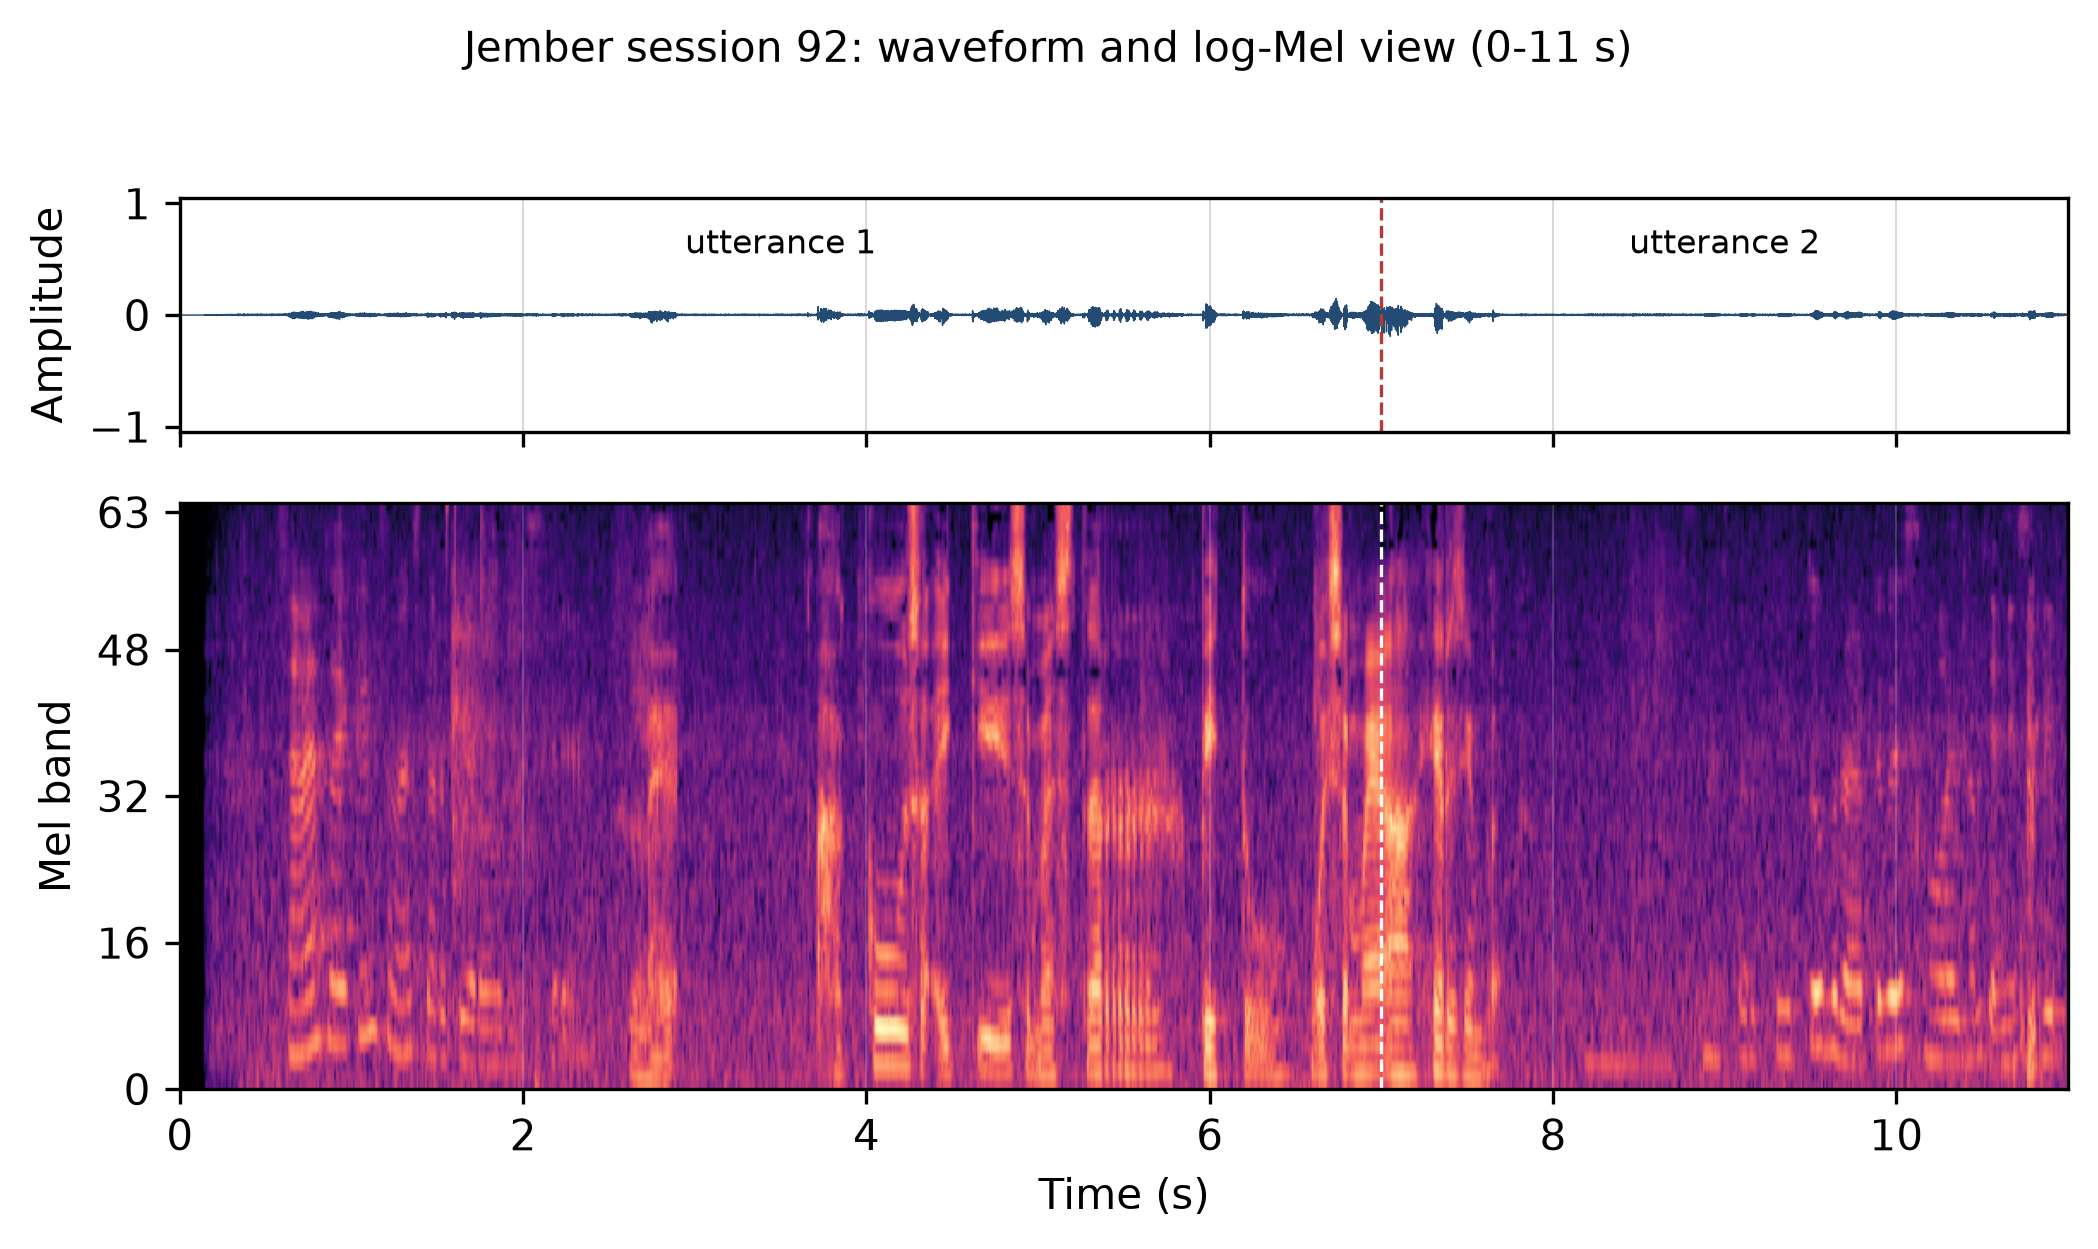
\includegraphics[width=\columnwidth]{paper_assets/jember_sample_spectrogram.png}
\caption{Waveform and 64-bin log-Mel representation of Jember session 92 from 0 to 11 s. The dashed line marks the transcript boundary between the two excerpts in Table~\ref{tab:sample}. The plot is an exploratory example; no performance claim is inferred from this segment.}
\label{fig:sample}
\end{figure}

\subsection{Exploratory Findings and Preparation}
The raw annotation rows have a median duration of 5 s. After grouping, the merged Jember chunks have a median duration of 26 s; 92.5\% fall between 15 and 32 s. The target development clips are similarly long, and the two conversations differ substantially in size. The data audit therefore retained source-row provenance, checked invalid timestamps and degenerate audio/text, converted audio to mono 16 kHz, and grouped neighboring segments only when the gap and maximum-duration conditions were met. Quality flags were recorded, but they were not used as an unvalidated domain-selection model.

The EDA changes how the results should be read. The development set is predominantly mixed speech, so it cannot support a strong Javanese-only claim. The vocabulary overlap is incomplete, so a better acoustic fit alone cannot remove every reference mismatch. The small number of conversations makes a conversation-held-out split more informative than a random clip split, but two conversations still provide narrow coverage.

\section{Methodology}
\subsection{End-to-End System}
Fig.~\ref{fig:pipeline} separates the completed competition path from the later offline research path. Both use the audited data and conversation-disjoint development design, but they use different Whisper sizes and fusion rules. Only the Turbo path is connected to the submitted leaderboard result.

\begin{figure*}[!t]
\centering
\resizebox{\textwidth}{!}{%
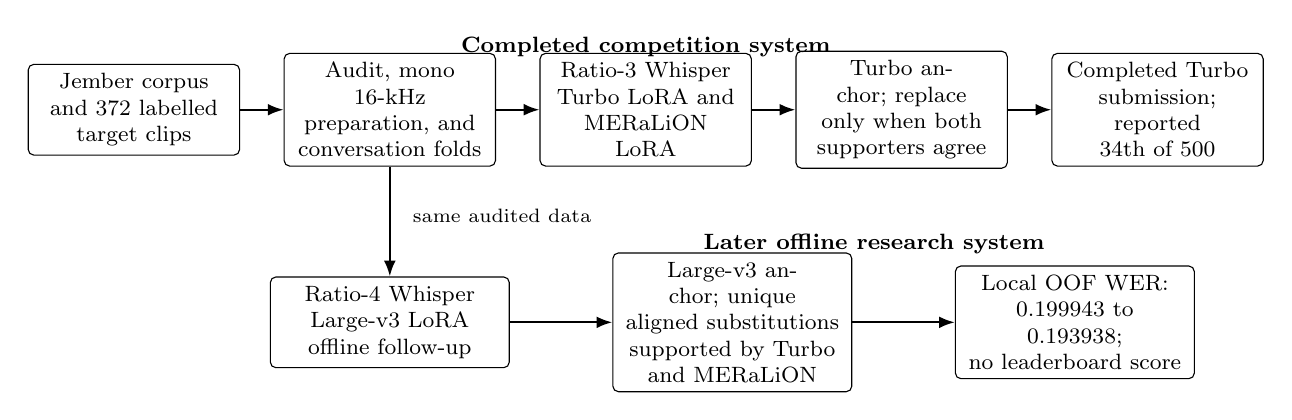
\begin{tikzpicture}[
  box/.style={draw,rounded corners=2pt,align=center,text width=2.45cm,minimum height=0.9cm,font=\footnotesize},
  research/.style={draw,rounded corners=2pt,align=center,text width=2.8cm,minimum height=0.9cm,font=\footnotesize},
  arr/.style={-{Latex[length=2mm]},thick}
]
\node[font=\footnotesize\bfseries] at (6.5,2.25) {Completed competition system};
\node[box] (data) at (0,1.45) {Jember corpus\\and 372 labelled\\target clips};
\node[box] (audit) at (3.25,1.45) {Audit, mono 16-kHz\\preparation, and\\conversation folds};
\node[box] (tmodels) at (6.5,1.45) {Ratio-3 Whisper\\Turbo LoRA and\\MERaLiON LoRA};
\node[box] (tfuse) at (9.75,1.45) {Turbo anchor; replace\\only when both\\supporters agree};
\node[box] (submit) at (13,1.45) {Completed Turbo\\submission; reported\\34th of 500};
\draw[arr] (data) -- (audit);
\draw[arr] (audit) -- (tmodels);
\draw[arr] (tmodels) -- (tfuse);
\draw[arr] (tfuse) -- (submit);

\node[research] (lmodel) at (3.25,-1.25) {Ratio-4 Whisper\\Large-v3 LoRA\\offline follow-up};
\node[research] (lfuse) at (7.6,-1.25) {Large-v3 anchor; unique\\aligned substitutions\\supported by Turbo\\and MERaLiON};
\node[research] (loof) at (11.95,-1.25) {Local OOF WER:\\0.199943 to 0.193938;\\no leaderboard score};
\draw[arr] (audit.south) -- (lmodel.north);
\draw[arr] (lmodel) -- (lfuse);
\draw[arr] (lfuse) -- (loof);
\node[font=\scriptsize,anchor=west] at (3.42,0.1) {same audited data};
\node[font=\footnotesize\bfseries] at (9.4,-0.25) {Later offline research system};
\end{tikzpicture}}
\caption{End-to-end study flow. The Large-v3 branch is a subsequent local experiment and is not the model credited with the final competition standing.}
\label{fig:pipeline}
\end{figure*}

\subsection{Evaluation and Error Metric}
Word error rate is computed as
\begin{equation}
\WER = \frac{S + D + I}{N},
\label{eq:wer}
\end{equation}
where \(S\), \(D\), and \(I\) are substitution, deletion, and insertion counts and \(N\) is the number of reference words. Aggregate WER is calculated from summed error and reference-word counts across folds:
\begin{equation}
\WER_{\mathrm{agg}} =
\frac{\sum_{k}(S_k+D_k+I_k)}{\sum_{k}N_k}.
\label{eq:aggregate}
\end{equation}
It is not the unweighted average of the two fold WERs. All WER values are fractions; for example, 0.193938 is 19.3938\%.

\subsection{Parameter-Efficient Adaptation}
For a pretrained projection \(W_0 \in \mathbb{R}^{d \times k}\), a low-rank update is
\begin{equation}
W = W_0 + \Delta W,\qquad
\Delta W = \frac{\alpha}{r}BA,
\label{eq:lora}
\end{equation}
where \(B \in \mathbb{R}^{d \times r}\), \(A \in \mathbb{R}^{r \times k}\), and \(r \ll \min(d,k)\). The base weights remain fixed while the low-rank matrices are trained.

The Whisper large-v3-turbo adaptation used rank \(r=32\), \(\alpha=64\), and dropout 0.05 over attention and feed-forward projections. Approximately 27.85 million of 836.73 million parameters were trainable. AdamW used a learning rate of \(3\times10^{-4}\), weight decay 0.01, gradient clipping at 1.0, 8\% warm-up, microbatch size 1, and accumulation over 16 steps. Competition examples were upweighted relative to Jember examples; ratios 2, 3, and 4 were compared, and the ratio-3 checkpoints were used in the completed conservative system.

MERaLiON-3-3B-ASR was adapted separately with decoder-side LoRA (rank 16, \(\alpha=32\), dropout 0.05). Its speech encoder and audio projector were frozen. This model was retained as a supporting hypothesis, not as the primary recognizer: its value was measured by what its output could safely correct, as well as by its standalone WER.

The later offline experiment used Whisper large-v3 with rank-16 LoRA, \(\alpha=32\), dropout 0.05, Indonesian conditioning, and ratio-4 sampling. The base ran in BF16 and the LoRA residuals in FP32. The model family, training ratio, and consensus rule differ from the submitted Turbo system and are reported separately.

\subsection{Conversation-Disjoint Validation}
The development set contains conversations 2 and 5. In Fold A, the model was trained on conversation 2 and the permitted Jember training chunks, then evaluated on conversation 5. Fold B reversed the target conversation roles. The 162-chunk Jember session-held-out split was used as a separate diagnostic. No Jember speaker IDs were available, and the diagnostic does not substitute for an independent target-domain test.

These folds test transfer across the two recorded conversations, not across a broad sample of speakers or settings. Since both folds were reused during model and rule selection, the aggregate scores are selected development estimates. This setup reduces direct clip leakage but does not remove adaptive overfitting to the small development set.

\subsection{Conservative Fusion Rules}
For the competition submission, the full-epoch Whisper Turbo output was the anchor. The half-epoch Turbo checkpoint and adapted MERaLiON supplied supporting outputs. Hypotheses were normalized for alignment, but the anchor's surface text was retained unless both supporting outputs agreed on the same short replacement. A replacement was eligible only if it contained at most three words, preserved token count, had unchanged context on each side, and contained no ordinary insertion or deletion. A single alternative could never replace the anchor by itself. A repetition safeguard was applied before fusion; its removals are counted separately from ordinary fusion edits.

The later Large-v3 consensus uses a distinct token-level procedure. For each anchor word, a supporter-to-anchor mapping is accepted only when that word maps uniquely across all minimum-cost alignments. Large-v3 is changed only if both supporters map the anchor word to the same normalized alternative. Ambiguous alignments, disagreements, and unchanged alternatives leave the anchor intact. This rule permits substitutions only and does not require an extra context-word test. We do not describe either rule as a new general fusion algorithm.

\section{Experimental Results}
\subsection{Conversation-Disjoint OOF Results}
Table~\ref{tab:oof} traces the main local development stages. The half-epoch Turbo model was a stronger initial single recognizer than adapted MERaLiON. Simple fusion gave only a small aggregate improvement and regressed on Fold B relative to the half-epoch Turbo model. The stricter three-output Turbo system improved both folds over that earlier anchor. The later Large-v3 consensus improved both folds again, but it is an offline follow-up rather than a competition result.

\begin{table*}[!t]
\caption{Conversation-disjoint OOF WER on the 372 labelled development clips. The two folds contain different numbers of reference words; aggregate WER is computed from pooled counts.}
\label{tab:oof}
\centering
\footnotesize
\begin{tabular}{lrrr}
\toprule
System & Fold A & Fold B & Aggregate \\
\midrule
Whisper Turbo, ratio-3 half epoch & 0.223634 & 0.204162 & 0.219674 \\
Adapted MERaLiON & 0.226578 & 0.220754 & 0.225393 \\
Simple Turbo--MERaLiON fusion & 0.218465 & 0.215129 & 0.217787 \\
Turbo three-output strict fusion & 0.209778 & 0.185321 & 0.204804 \\
Whisper Large-v3 standalone & 0.205542 & 0.178009 & 0.199943 \\
Large-v3 with unambiguous consensus & 0.199368 & 0.172666 & 0.193938 \\
\bottomrule
\end{tabular}
\end{table*}

The selected Large-v3 consensus reduced aggregate WER by 0.006005, or approximately 3.00\% relative to the Large-v3 anchor. The improvement was present on both folds. To assess whether this gain is statistically meaningful, we conducted a paired Wilcoxon signed-rank test and non-parametric bootstrap resampling (1,000 rounds) across all 372 development clips. Utterance-level analysis shows that the consensus policy improved 110 clips (29.6\%), regressed 34 clips (9.1\%), and left 228 clips unchanged (a 3.24$\times$ win-to-loss ratio). The paired signed-rank test confirms that the reduction is highly significant ($W = 8218.0$, $p = 1.12 \times 10^{-9}$). Furthermore, the 95\% bootstrap confidence interval on the absolute WER reduction is $[+0.429\%, +0.787\%]$ (relative $[+2.14\%, +3.94\%]$), strictly excluding zero. The Large-v3 adaptation used the target development conversations in opposite train/test directions, so these predictions are out of fold but not independent of model selection.

\subsection{Leaderboard Outcome}
The submitted artifact used the conservative Turbo system, not the later Large-v3 research candidate. The project record retains two displayed score columns but the supplied screenshot does not preserve their headings. Table~\ref{tab:leaderboard} therefore labels the values by display order rather than assigning an unverified metric name. The final values were 0.2712 and 0.2743. The team reports a final standing of 34th among 500 entries.\footnote{The rank was supplied by the team. A timestamped public leaderboard record or official result URL should be retained with the final submission materials.}

\begin{table*}[!t]
\caption{Reported competition progression. The archived screenshot omits the two score-column headings, so the values below are transcribed without assigning a metric label.}
\label{tab:leaderboard}
\centering
\footnotesize
\begin{tabular}{lrr}
\toprule
Submission stage & Displayed column 1 & Displayed column 2 \\
\midrule
Completed entry 1 (system label unavailable) & 0.4273 & 0.4234 \\
Completed entry 2 (system label unavailable) & 0.4140 & 0.4123 \\
Legacy competition submission & 0.4009 & 0.3963 \\
Adapted Whisper Turbo & 0.2862 & 0.2914 \\
Three-model protected fusion & 0.2786 & 0.2837 \\
Final conservative Turbo fusion & \textbf{0.2712} & \textbf{0.2743} \\
\midrule
Final team-reported position & \multicolumn{2}{c}{\textbf{34th of 500 entries}} \\
\bottomrule
\end{tabular}
\end{table*}

The final conservative package completed CUDA inference in approximately 1,840 s (30.7 min) according to the saved run record. The later Large-v3 package has no supplied competition score. Its local OOF WER must not be used to imply a new leaderboard result.

\section{Ablation and Variation Studies}
The submitted Turbo variants expose a practical trade-off between score and edit risk. A broader rule achieved a lower aggregate WER than the selected strict rule, but it made more edits and introduced ordinary insertions and deletions. The conservative rule was selected for bounded behavior, not because it had the lowest WER.

For the later Large-v3 study, unambiguous boundary consensus outperformed the tested context and short insertion/deletion variants in Table~\ref{tab:variants}. N-best rescoring produced the lowest numeric WER, but its gain was only nine word errors, an aggregate change of 0.000515. This fell below the predeclared 0.0015 material-gain threshold; N-best also added insertion/deletion edits and decoding complexity, so it was not selected.

\begin{table*}[!t]
\caption{Selected variation and ablation results. Turbo submission variants and Large-v3 research variants use different anchors and must not be interpreted as a single controlled experiment.}
\label{tab:variants}
\centering
\footnotesize
\begin{tabular}{p{4.0cm}r p{4.0cm} p{5.0cm}}
\toprule
Variant & Aggregate WER & Edit profile & Interpretation \\
\midrule
Turbo, broader exact-support edits & 0.203660 & 157 substitutions, 21 insertions, 17 deletions & Numerically lower than the strict variant; more edit types and 61 more word edits. \\
Turbo, strict substitution-only (submitted) & 0.204804 & 134 substitutions, no ordinary insertions/deletions & Selected risk-control choice; not the minimum-WER Turbo variant. \\
Large-v3 standalone anchor & 0.199943 & No fusion edits & Reference point for the later offline study. \\
Large-v3, Turbo and MERaLiON, context variant & 0.196454 & Unambiguous aligned-word corrections with context check & Lower than the anchor, but weaker than boundary consensus. \\
Large-v3, Turbo and MERaLiON, boundary consensus & \textbf{0.193938} & 277 substitutions in 267 spans; no ordinary insertions/deletions & Selected local research rule; changed 173 of 372 clips. \\
Large-v3 with short insertion/deletion edits & 0.195939 & 210 substitutions, 14 insertions, 19 deletions & Additional edit operations did not improve WER. \\
Large-v3 with two Turbo supporters & 0.200172 & Strict support rule & Replacing MERaLiON with a second Turbo checkpoint regressed both folds. \\
Cross-fold logistic edit gate & 0.195825 & Learned edit decision & Rejected; weaker than the deterministic consensus. \\
Large-v3 targeted N-best rescoring & 0.193423 & 305 substitutions, 2 insertions, 8 deletions & Nine-word gain; below material-gain threshold and added complexity. \\
\bottomrule
\end{tabular}
\end{table*}

The early Turbo variation study also compared language conditioning and competition-to-Jember sampling ratios. Ratio-3 Indonesian conditioning was selected for the first submission because it kept the worst of the two target folds lower than the tested ratio-4 full checkpoint, even though ratio 4 had a slightly lower aggregate WER. Forced Javanese conditioning improved one fold while substantially worsening the other. This is why the paper reports fold-level results and does not select a model from a single aggregate number alone.

\section{Qualitative Error Analysis}
The cached OOF examples show both sides of the agreement rule. In one Fold A clip, the anchor phrase "beberapa kali pengin" was changed to "beberapa kali pengen"; whole-clip WER fell from 0.1875 to 0.1458. In another Fold A clip, "nggak" was changed to "gak" and whole-clip WER rose from 0.2174 to 0.2391. These references were used only after inference to classify the examples. Agreement reduced the number of eligible edits, but did not guarantee that a replacement matched the reference. The orthographic differences also show why a consensus transcript can be acoustically plausible yet score worse under exact reference spelling.

\section{Discussion}
Three observations guide the next iteration. First, adaptation mattered more than adding recognizers indiscriminately: the development process moved from heterogeneous voting to a stronger target-adapted anchor. Second, a supporting model's standalone score did not fully describe its value. Adapted MERaLiON was weaker than the Turbo anchor on aggregate WER, yet its output helped identify corrections when it agreed with the other supporter. Third, the edit policy is part of the system's risk profile. The selected Turbo rule accepted 61 fewer ordinary word edits than the broader variant, while the later Large-v3 rule improved both OOF folds.

The gap between local and competition results remains important. The early metadata-blind full-development replay was approximately 0.2058, while a preceding completed competition entry displayed 0.4009 in one score column. These are different evaluation records, and the available materials do not establish a one-to-one metric mapping or a definitive cause for the discrepancy. It triggered the shift toward simpler inference and stronger deployment checks. Possible contributors include target-distribution shift, annotation conventions, model/runtime differences, and the very small number of development conversations. These explanations remain hypotheses.

\section{Limitations and Future Work}
This is a focused case study with several limits. The target development set contains only two conversations and four speakers, with only 20 Indonesian-only clips and no Javanese-only clips. Repeated use of the same folds during model selection makes the OOF estimates adaptive rather than untouched test results. While paired non-parametric tests ($p = 1.12 \times 10^{-9}$) and bootstrap confidence intervals now confirm the statistical significance of the local OOF gain, Jember remains a supplementary corpus with different dialectal coverage and no speaker IDs; its session-held-out diagnostic is not a substitute for a larger independent target sample.

The Large-v3 consensus was evaluated locally only. It has no measured leaderboard result and cannot be credited with the reported rank. The submission screenshot available while preparing this manuscript omitted score-column headings; the two values and team-reported rank should be paired with an archived official result page before journal submission. The related-work section is a focused journal-paper review rather than a systematic review, so the gap should be revisited before claiming novelty for a specific venue.

Future work should freeze the complete system and edit policy before evaluation on additional independent conversations and speakers. It should include Javanese-only material and compare consensus against quality-estimation-guided and voting baselines under identical decoding and normalization. Community review of spelling conventions could separate acoustic recognition failures from orthographic disagreement. A future Large-v3 leaderboard run, if allowed by contest rules, should be reported as a new measurement rather than inferred from OOF performance.

\section{Conclusion}
We documented a complete Indonesian--Javanese ASR competition workflow from corpus audit and EDA to model adaptation, conversation-disjoint evaluation, conservative fusion, and deployment. The completed Turbo submission finished with the reported displayed values 0.2712 and 0.2743 and a team-reported 34th-place position among 500 entries. A later Large-v3 system reduced local aggregate OOF WER from 0.199943 to 0.193938 using unambiguous two-supporter word substitutions, but that system has no competition result. The evidence supports a practical lesson for future contests: adapt a strong anchor, evaluate by conversation, preserve the anchor unless model outputs agree, and keep every local, OOD, and leaderboard measurement distinct.

\section*{Acknowledgment}
The authors acknowledge the Lost in Transcription organizers and the providers of the supplementary Jember speech corpus.

\begin{thebibliography}{00}
\bibitem{mustafa}
M. B. Mustafa, M. A. Yusoof, H. K. Khalaf, A. A. R. M. Abushariah, M. L. M. Kiah, H. N. Ting, and S. Muthaiyah, "Code-switching in automatic speech recognition: The issues and future directions," \emph{Applied Sciences}, vol. 12, no. 19, Art. no. 9541, 2022, doi: 10.3390/app12199541.

\bibitem{hamed}
I. Hamed, P. Denisov, C.-Y. Li, M. Elmahdy, S. Abdennadher, and N. T. Vu, "Investigations on speech recognition systems for low-resource dialectal Arabic--English code-switching speech," \emph{Computer Speech \& Language}, vol. 72, Art. no. 101278, 2022, doi: 10.1016/j.csl.2021.101278.

\bibitem{jain}
P. Jain and A. Bhowmick, "Analyzing code-switching scenarios in India's diverse linguistic landscape using end-to-end ASR systems with VITB-HEBiC," \emph{Computers \& Electrical Engineering}, vol. 122, Art. no. 109978, Mar. 2025, doi: 10.1016/j.compeleceng.2024.109978.

\bibitem{raharjo}
A. Raharjo and A. Zahra, "Javanese and Sundanese speech recognition using Whisper," \emph{Computer Science and Information Technologies}, vol. 6, no. 3, pp. 253--261, Nov. 2025, doi: 10.11591/csit.v6i3.p253-261.

\bibitem{setiawan}
J. Setiawan, A. Luthfiarta, A. Nugraha, R. Rismiyati, J. C. Bastiaans, and Y. D. Novandian, "Automatic speech recognition for Javanese language using Wav2Vec 2.0 with finetuning," \emph{Jurnal Nasional Teknologi dan Sistem Informasi}, vol. 12, no. 1, pp. 1--9, Apr. 2026, doi: 10.25077/TEKNOSI.v12i1.2026.1-9.

\bibitem{liu}
Y. Liu, X. Yang, and D. Qu, "Exploration of Whisper fine-tuning strategies for low-resource ASR," \emph{EURASIP Journal on Audio, Speech, and Music Processing}, vol. 2024, Art. no. 29, 2024, doi: 10.1186/s13636-024-00349-3.

\bibitem{jalalvand}
S. Jalalvand, M. Negri, D. Falavigna, M. Matassoni, and M. Turchi, "Automatic quality estimation for ASR system combination," \emph{Computer Speech \& Language}, vol. 47, pp. 214--239, Jan. 2018, doi: 10.1016/j.csl.2017.06.003.
\end{thebibliography}

\end{document}
